\section{SOLUCIÓN PROPUESTA}

La solución propuesta consiste en un modelo computacional de aprendizaje adaptativo para la enseñanza de teoría musical, diseñado para recomendar dinámicamente actividades de acuerdo con el progreso individual del estudiante y la estructura pedagógica del dominio. El modelo se estructura sobre tres componentes complementarios: (i) un Grafo de Conocimiento Dirigido Acíclico (DAG), encargado de representar explícitamente las dependencias entre los conceptos musicales; (ii) un agente basado en \textit{Deep Reinforcement Learning} (DRL), responsable de aprender una política de recomendación adaptativa; y (iii) la plataforma \textbf{SheetMusic}, que implementa el modelo y proporciona las funcionalidades necesarias para estudiantes y docentes.

El modelo fue implementado en \textbf{SheetMusic}, una plataforma web progresiva que articula la experiencia de aprendizaje del estudiante, las herramientas de seguimiento pedagógico del docente y un microservicio inteligente encargado de generar las recomendaciones. La separación entre la representación del conocimiento, el motor de decisión y la plataforma permite desacoplar la lógica adaptativa de los componentes de presentación, persistencia y procesamiento inteligente.

%--------------------------------------------------------
\subsection{Modelo Funcional de SheetMusic}

La implementación del modelo de aprendizaje adaptativo se materializa mediante \textbf{SheetMusic}, una plataforma web progresiva diseñada para apoyar tanto el proceso de aprendizaje de los estudiantes como el seguimiento pedagógico realizado por los docentes. Desde una perspectiva funcional, la plataforma define dos actores principales: el \textit{Estudiante}, quien interactúa con el sistema mediante actividades de estudio, práctica y seguimiento de su progreso; y el \textit{Profesor}, responsable de la gestión de cursos, la administración de estudiantes, la asignación de actividades y el monitoreo del desempeño académico.

La Figura~\ref{fig:casos_uso} presenta la visión funcional de SheetMusic mediante un diagrama de casos de uso unificado, mostrando las principales funcionalidades disponibles para ambos perfiles de usuario. Esta visión funcional establece el contexto operativo sobre el cual se implementa el modelo computacional de aprendizaje adaptativo descrito en las siguientes subsecciones.

\begin{figure}[htbp]
    \centering
    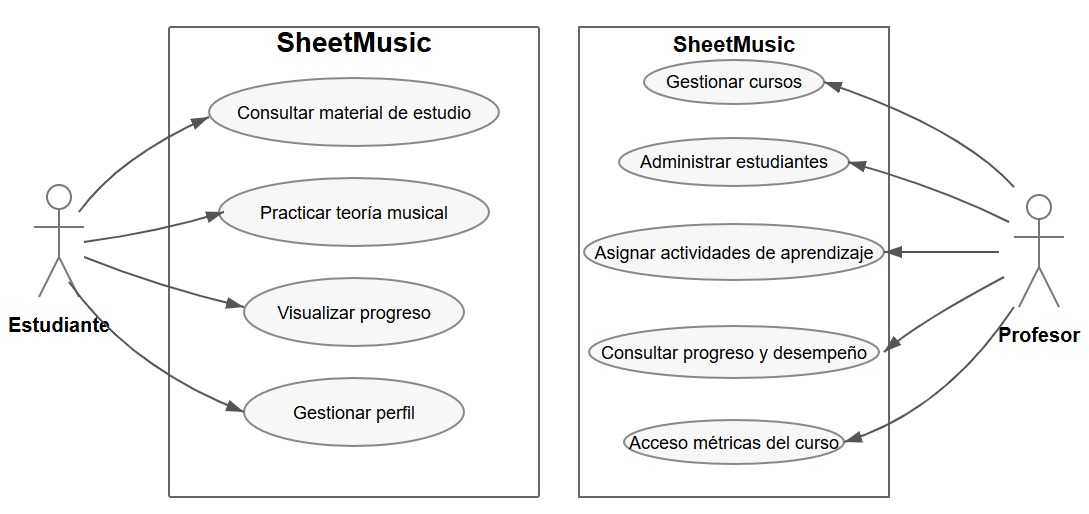
\includegraphics[width=0.3\textwidth]{Imagenes/caso_uso.jpeg}
    \caption{Modelo funcional de la plataforma SheetMusic, mostrando los principales casos de uso para los perfiles de Estudiante y Profesor.}
    \label{fig:casos_uso}
\end{figure}

%--------------------------------------------------------
\subsection{Grafo de Conocimiento Musical}

La representación explícita del dominio de conocimiento constituye uno de los pilares del modelo de aprendizaje adaptativo propuesto, ya que permite formalizar computacionalmente las relaciones pedagógicas existentes entre los distintos contenidos de teoría musical. En lugar de organizar los ejercicios mediante una secuencia fija, el modelo representa el dominio como una estructura de dependencias que permite identificar prerrequisitos, establecer trayectorias de aprendizaje coherentes y restringir las recomendaciones a actividades pedagógicamente válidas~\cite{manrique2019kg}.

Con este propósito, el dominio de la teoría musical se formalizó mediante un \textbf{Grafo de Conocimiento Dirigido Acíclico (DAG)} definido como:

\begin{equation}
G=(V,E)
\end{equation}

donde $V$ representa el conjunto de unidades de conocimiento (nodos) y $E$ el conjunto de aristas dirigidas que modelan las relaciones de dependencia pedagógica entre dichos conceptos. En la implementación completa del sistema, el grafo está compuesto por 23 unidades de conocimiento distribuidas en cinco niveles de dificultad y 29 relaciones de dependencia. Estas dependencias representan prerrequisitos recomendados para favorecer una progresión lógica del aprendizaje, aunque no constituyen restricciones absolutas, ya que un estudiante puede acceder a contenidos posteriores cuando demuestra un nivel de dominio suficiente durante el proceso de evaluación adaptativa.

Con el propósito de facilitar la validación experimental del modelo, en este trabajo se empleó un subgrafo compuesto por cuatro unidades de conocimiento fundamentales de teoría musical: \textit{Notas y Ritmo}, \textit{Intervalos}, \textit{Escalas Mayores y Menores} y \textit{Acordes (Tríadas)}. Estos conceptos permiten representar las principales relaciones de dependencia pedagógica presentes en el dominio y constituyen una base suficiente para evaluar el comportamiento del sistema de recomendación.

\begin{figure}[htbp]
    \centering
    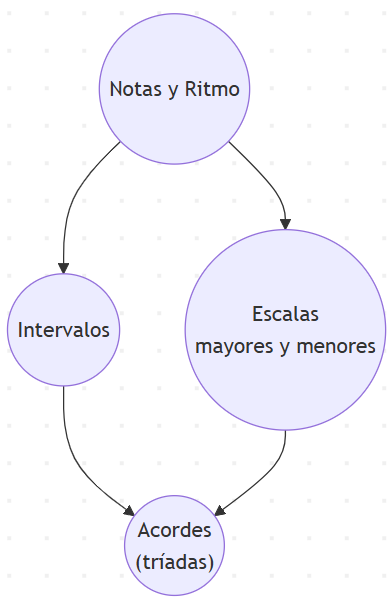
\includegraphics[width=0.15\textwidth]{Imagenes/grafo_dag.png}
    \caption{Subgrafo del Grafo de Conocimiento Musical utilizado durante la validación experimental. Cada nodo representa una unidad de conocimiento y cada arista dirigida representa una relación de prerrequisito pedagógico entre conceptos.}
    \label{fig:dag}
\end{figure}

La Figura~\ref{fig:dag} muestra el subgrafo utilizado durante la validación. En esta representación, las aristas dirigidas indican los prerrequisitos pedagógicos entre los distintos conceptos, permitiendo establecer una progresión lógica del aprendizaje desde contenidos básicos hacia unidades de mayor complejidad.

Para que el agente de recomendación pueda determinar las actividades disponibles en cada instante del proceso de aprendizaje, cada nodo del grafo mantiene un estado asociado al progreso alcanzado por el estudiante. Dicho estado puede corresponder a una unidad bloqueada (\textit{locked}), disponible (\textit{available}), en desarrollo (\textit{active}) o completada (\textit{done}), según la siguiente definición:

\begin{equation}
State(v_i)=
\begin{cases}
\text{locked}, & \exists u \in Pred(v_i)\mid Prog(u)\neq\text{done}\\
\text{done}, & Prog(v_i)=\text{done}\\
\text{active}, & Prog(v_i)=\text{in\_progress}\\
\text{available}, & \text{en otro caso}
\end{cases}
\end{equation}

Esta representación no determina directamente cuál será la siguiente actividad recomendada, sino que define el conjunto de actividades pedagógicamente válidas para el estado actual del estudiante. Sobre este espacio de decisión opera posteriormente el agente basado en \textit{Deep Reinforcement Learning}, encargado de seleccionar la recomendación que maximiza el progreso esperado del proceso de aprendizaje.

%--------------------------------------------------------
\subsection{Modelo de Recomendación Basado en Deep Reinforcement Learning}

Una vez representado el dominio de conocimiento mediante el Grafo de Conocimiento Musical, el problema de recomendación adaptativa se modela como un proceso de decisión secuencial, donde un agente basado en \textit{Deep Reinforcement Learning} (DRL) selecciona dinámicamente la siguiente actividad de aprendizaje considerando el estado actual del estudiante y las restricciones pedagógicas definidas por el DAG. El objetivo del agente consiste en aprender una política de recomendación que maximice el progreso esperado del estudiante, equilibrando la consolidación de conocimientos, la exploración de nuevos contenidos y la dificultad de los ejercicios.

La implementación del agente se desarrolló utilizando \textit{Stable-Baselines3} (versión 2.0.1) sobre \textit{Gymnasium} (versión 1.2.0), siguiendo el esquema clásico de interacción \textit{agent-environment loop}, donde el agente observa el estado del estudiante, selecciona una actividad, recibe retroalimentación y actualiza iterativamente su política de decisión.

\subsubsection{Entorno de Aprendizaje}

El entorno de entrenamiento, denominado \texttt{MusicLearningEnv}, fue implementado como una subclase de \texttt{gymnasium.Env}. Cada interacción corresponde a un episodio donde el agente selecciona un ejercicio de teoría musical, observa la respuesta del estudiante y recibe una recompensa asociada al impacto pedagógico de dicha decisión.

\subsubsection{Espacio de Observaciones}

El estado del estudiante se representa mediante la clase \texttt{UserState}, la cual encapsula la información necesaria para describir su situación de aprendizaje. Entre los atributos considerados se encuentran: \textbf{knowledge} (nivel de dominio de cada concepto), \textbf{accuracy} (precisión histórica), \textbf{attempts} (cantidad de intentos por concepto), \textbf{streak} (racha de aciertos o errores), \textbf{last\_exercise\_difficulty} (última dificultad presentada), \textbf{time\_since\_last\_practice} (tiempo desde la última práctica) y \textbf{recent\_performance\_trend} (tendencia reciente de desempeño).

Para el proceso de inferencia, el nivel de dominio se discretiza utilizando un umbral de proficiencia de 0.5:

\begin{equation}
o_i=
\begin{cases}
1, & \text{si } proficiency_i \ge 0.5\\
0, & \text{en otro caso}
\end{cases}
\end{equation}

obteniéndose un vector binario (\texttt{MultiBinary}) que resume el estado de conocimiento del estudiante y constituye la entrada utilizada por el agente DRL.

\subsubsection{Espacio de Acciones}

El espacio de acciones se define como un conjunto discreto (\texttt{Discrete(N)}), donde cada acción corresponde a un ejercicio específico de teoría musical asociado a uno de los nodos del DAG mediante la estructura \texttt{skill\_mapping}. Esta representación desacopla el modelo de aprendizaje del conjunto de ejercicios disponible, permitiendo incorporar nuevos contenidos o eliminar ejercicios existentes sin modificar la estructura del agente.

\subsubsection{Función de Recompensa}

La política del agente se aprende mediante la maximización de una recompensa acumulada que refleja el equilibrio entre el progreso pedagógico del estudiante y la calidad de las recomendaciones generadas. Para ello, se definió una función de recompensa compuesta por incentivos y penalizaciones, orientada a favorecer trayectorias de aprendizaje efectivas y evitar decisiones pedagógicamente inadecuadas.

\begin{equation}
\begin{aligned}
R =\;&
1.0\,\mathbb{I}(\text{correcto})
+0.5\,\mathbb{I}(\text{mejoría}) \\
&+0.5\,\mathbb{I}\!\left(
|d-d^{*}|\le1
\right)
-0.3\,\mathbb{I}\!\left(
|d-d^{*}|>2
\right) \\
&+0.2\,\mathbb{I}(\text{nodo poco practicado})
+0.1\,\mathbb{I}(\text{ejercicio nuevo})
\end{aligned}
\end{equation}

donde $d^{*}=proficiency\times10$ representa la dificultad esperada para el nivel actual del estudiante.

Los términos positivos incentivan respuestas correctas, mejoras respecto al desempeño previo, ejercicios cercanos a la zona de desarrollo proximal, exploración de contenidos poco practicados y variedad en las actividades recomendadas. Por otra parte, el agente recibe penalizaciones cuando recomienda ejercicios cuya dificultad resulta inadecuada para el nivel del estudiante, cuando repite innecesariamente un mismo ejercicio o cuando intenta acceder a contenidos cuyos prerrequisitos pedagógicos definidos por el DAG aún no han sido alcanzados. En consecuencia, el agente aprende simultáneamente a maximizar el progreso esperado del estudiante y a minimizar recomendaciones pedagógicamente inconsistentes.

\subsubsection{Selección del Algoritmo de Aprendizaje}

Con el objetivo de determinar el algoritmo más adecuado para el problema de recomendación adaptativa, se evaluaron dos enfoques ampliamente utilizados en Deep Reinforcement Learning: \textit{Deep Q-Network} (DQN) y \textit{Proximal Policy Optimization} (PPO).

Durante las pruebas experimentales, DQN presentó una convergencia inicial más rápida, alcanzando políticas aceptables después de aproximadamente 120 episodios. Sin embargo, mostró una tendencia a favorecer acciones previamente exitosas, reduciendo la exploración de nuevos contenidos y generando políticas excesivamente conservadoras.

Por el contrario, PPO presentó una convergencia ligeramente más lenta (150--180 episodios), pero desarrolló políticas considerablemente más estables, manteniendo un mejor equilibrio entre exploración y explotación. Además, su arquitectura \textit{actor-critic} y el uso de políticas estocásticas permitieron obtener recomendaciones menos predecibles y más consistentes con la variabilidad esperada en procesos educativos adaptativos. Por estas razones, PPO fue seleccionado como algoritmo de recomendación del sistema.

\subsubsection{Estrategia de Entrenamiento}

Debido a que durante las primeras etapas del proyecto no se disponía de datos históricos de interacción suficientes para entrenar el agente mediante aprendizaje por refuerzo, se diseñó una estrategia de entrenamiento en dos etapas.

En primer lugar, se aplicó un cuestionario a estudiantes de enseñanza media para estimar perfiles iniciales de conocimiento y parámetros de aprendizaje. A partir de estos datos se implementó un simulador probabilístico denominado \texttt{SyntheticStudent}, capaz de generar trayectorias sintéticas de aprendizaje para distintos perfiles de estudiantes.

Posteriormente, el entrenamiento se realizó mediante un esquema híbrido. Inicialmente se aplicó \textit{Behavior Cloning}, técnica de aprendizaje por imitación utilizada para inicializar una política a partir de demostraciones o decisiones de referencia~\cite{osa2018imitation}. En este trabajo, dicha política inicial fue construida utilizando criterios pedagógicos definidos por expertos en teoría musical. Sobre esta política base se ejecutó posteriormente el entrenamiento mediante PPO utilizando aproximadamente 200\,000 interacciones simuladas, permitiendo refinar progresivamente la política de recomendación hasta obtener un comportamiento estable y adaptativo.

Este enfoque híbrido combina conocimiento pedagógico explícito, incorporado inicialmente mediante \textit{Behavior Cloning}, con la capacidad de optimización autónoma proporcionada por \textit{Deep Reinforcement Learning}. Como resultado, el agente inicia el proceso de aprendizaje a partir de una política consistente con criterios pedagógicos definidos por expertos y posteriormente la refina mediante interacción con el entorno, obteniendo recomendaciones progresivamente más adaptativas y robustas.

%--------------------------------------------------------
\subsection{Arquitectura Distribuida}

La implementación del modelo de aprendizaje adaptativo propuesto se materializa mediante una arquitectura distribuida basada en microservicios, diseñada para desacoplar la interfaz de usuario, la gestión de datos y el motor de inteligencia artificial encargado de generar las recomendaciones adaptativas. Esta separación permite que cada componente evolucione de manera independiente, facilita el escalamiento horizontal del sistema y posibilita incorporar mejoras al modelo de aprendizaje sin modificar la plataforma utilizada por estudiantes y docentes \cite{charland_mobile_2011,flutter_vs_ionic_2023}.

La Figura~\ref{fig:arquitectura} presenta la arquitectura general de \textbf{SheetMusic}, organizada en tres capas principales: una capa cliente responsable de la interacción con los usuarios, una capa de servicios encargada de la autenticación y persistencia de la información académica, y una capa de inteligencia donde se ejecuta el modelo basado en \textit{Deep Reinforcement Learning}.

%--------------------------------------------------------
% FIGURA 3
% Arquitectura General
%--------------------------------------------------------

\begin{figure}[htbp]
    \centering
    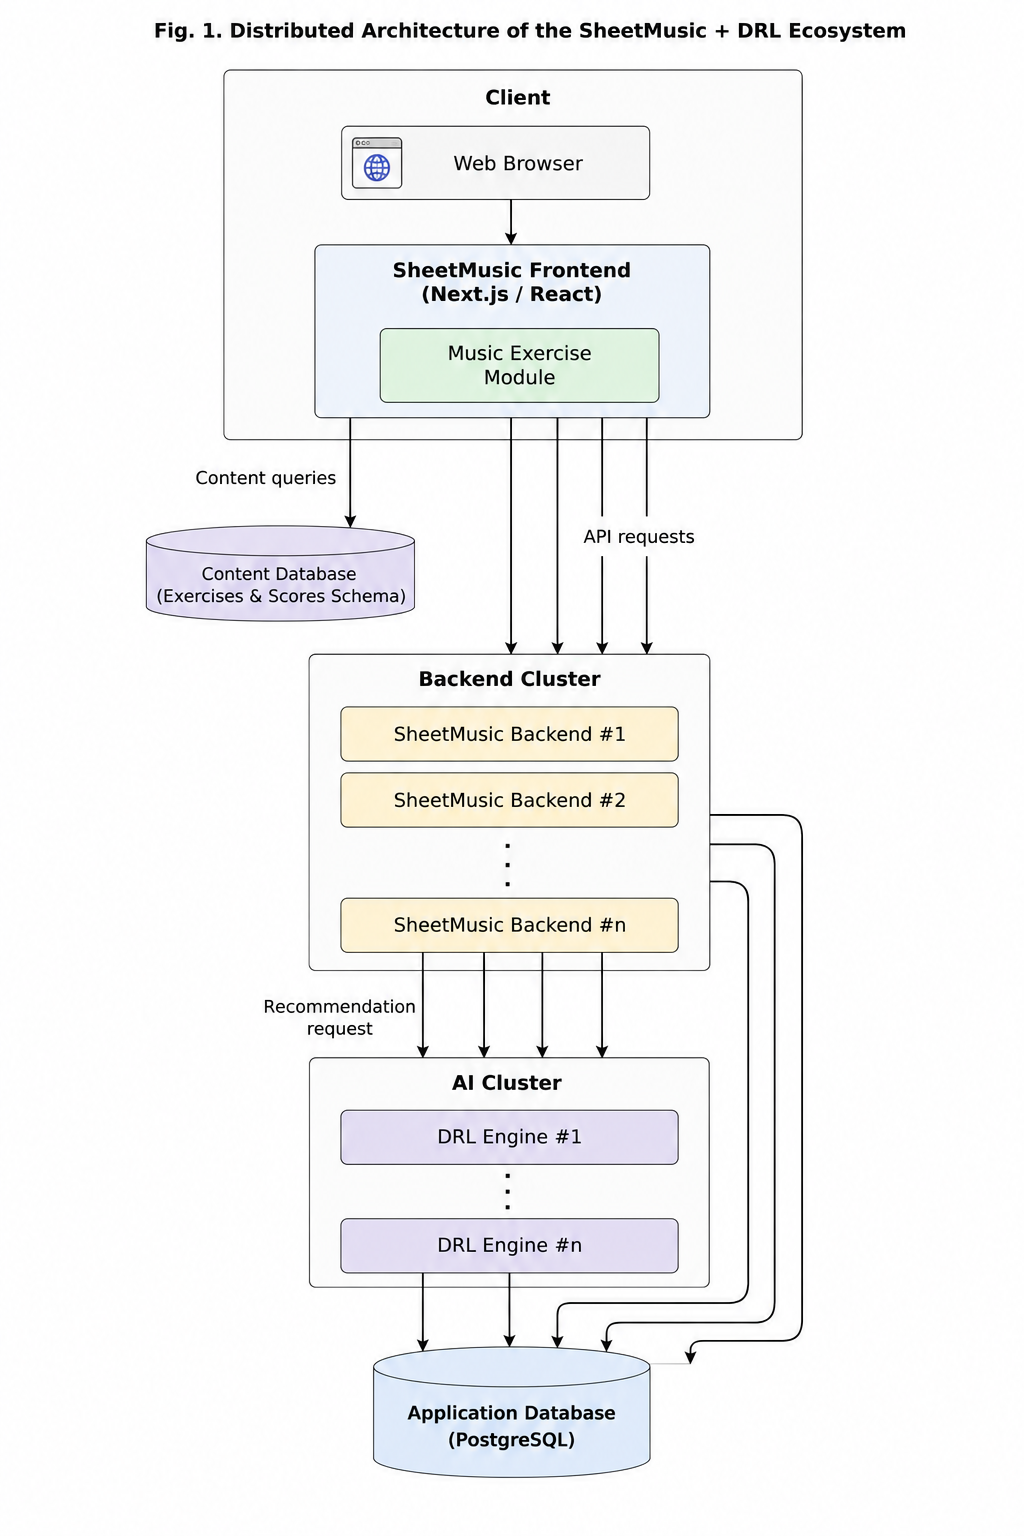
\includegraphics[width=0.3\textwidth]{Imagenes/fig_arch_system.png}
    \caption{Arquitectura distribuida de SheetMusic y sus principales componentes.}
    \label{fig:arquitectura}
\end{figure}

\subsubsection{Componentes de la Arquitectura}

La arquitectura propuesta está compuesta por tres componentes principales:

\begin{itemize}

\item \textbf{Capa Cliente.} Implementada como una \textit{Progressive Web Application} (PWA) utilizando Ionic React y Capacitor, proporciona la interfaz mediante la cual estudiantes y docentes acceden al material de estudio, resuelven ejercicios, consultan su progreso académico y administran las actividades del curso.

\item \textbf{Capa de Servicios.} Implementada sobre Supabase y PostgreSQL, administra la autenticación de usuarios mediante \textit{JSON Web Tokens} (JWT), el almacenamiento del historial académico y la comunicación con la aplicación cliente mediante procedimientos remotos (RPC). Asimismo, aplica políticas de seguridad basadas en \textit{Row Level Security} (RLS), garantizando el aislamiento de la información entre estudiantes y docentes \cite{supabase_docs_2024}.

\item \textbf{Motor de Inteligencia.} Implementado como un microservicio independiente utilizando FastAPI, PyTorch y Stable-Baselines3, recibe el estado actualizado del estudiante, ejecuta el agente basado en PPO y retorna la recomendación del siguiente ejercicio junto con su nivel de dificultad adaptativo.

\end{itemize}

\subsubsection{Flujo de Interacción Distribuida}

La arquitectura implementa dos flujos principales de interacción entre sus componentes. El primero corresponde al acceso al contenido pedagógico y el segundo al proceso de inferencia adaptativa realizado por el agente basado en Deep Reinforcement Learning.

La Figura~\ref{fig:contenido} ilustra el flujo utilizado para el renderizado dinámico del material de aprendizaje. Cuando un estudiante accede a una unidad de conocimiento, la aplicación cliente solicita el contenido correspondiente mediante procedimientos remotos (RPC) al backend de Supabase. La información es recuperada desde la base de datos utilizando objetos JSONB, los cuales son interpretados por el cliente para construir dinámicamente la interfaz de aprendizaje, incluyendo recursos multimedia, barras de progreso, tarjetas de conceptos clave y elementos de gamificación.

%--------------------------------------------------------
% FIGURA 4
%--------------------------------------------------------

\begin{figure}[htbp]
    \centering
    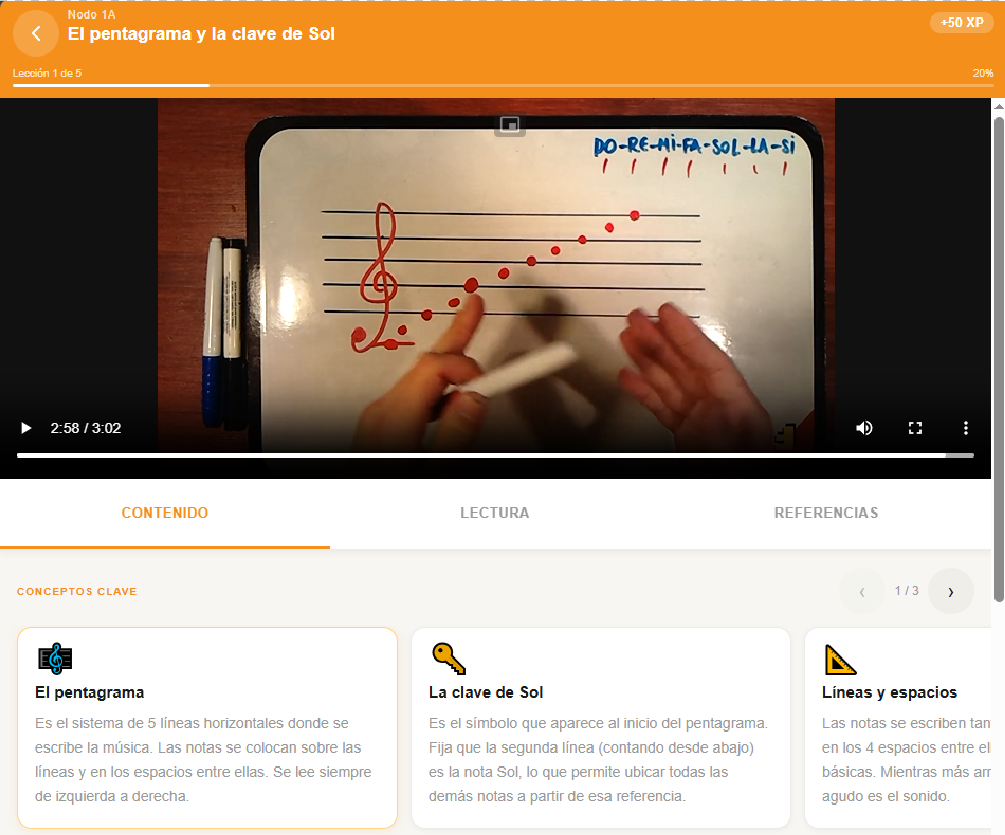
\includegraphics[width=0.3\textwidth]{Imagenes/MaterialAprendizajeFrontend.png}
    \caption{Renderizado dinámico del contenido pedagógico utilizando objetos JSONB recuperados desde el backend.}
    \label{fig:contenido}
\end{figure}

Una vez finalizada una actividad, se inicia el segundo flujo de interacción, correspondiente al proceso de recomendación adaptativa. Como se observa en la Figura~\ref{fig:inferencia}, el cliente envía el resultado del ejercicio al backend, el cual valida la sesión del usuario, actualiza el historial académico y construye el vector de observaciones requerido por el agente DRL. Posteriormente, el microservicio de inteligencia ejecuta el modelo PPO, determina la siguiente recomendación considerando el estado del estudiante y las restricciones impuestas por el Grafo de Conocimiento Musical, y retorna la respuesta al backend. Finalmente, la plataforma presenta al estudiante el siguiente ejercicio junto con su nivel de dificultad adaptativo, completando el ciclo de aprendizaje.

%--------------------------------------------------------
% FIGURA 5
%--------------------------------------------------------

\begin{figure}[htbp]
    \centering
    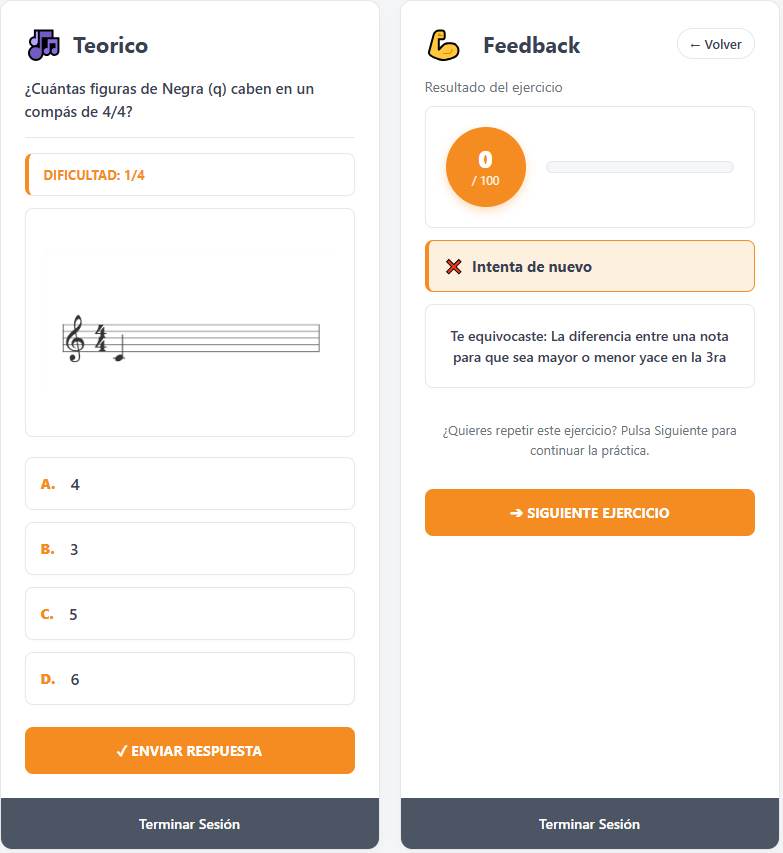
\includegraphics[width=0.3\textwidth]{Imagenes/frontend_ejercicio.png}
    \caption{Flujo distribuido de inferencia entre el cliente, el backend y el motor de Deep Reinforcement Learning.}
    \label{fig:inferencia}
\end{figure}

La arquitectura distribuida propuesta desacopla completamente la representación del conocimiento (DAG), el proceso de toma de decisiones basado en Deep Reinforcement Learning y la interfaz utilizada por estudiantes y docentes. Como consecuencia, nuevas estrategias de recomendación, funciones de recompensa o modelos de aprendizaje pueden incorporarse al sistema sin modificar la plataforma cliente, favoreciendo la mantenibilidad, escalabilidad y evolución futura de \textbf{SheetMusic}.
